\documentclass[12pt]{article}
\usepackage{fullpage,graphicx,psfrag,amsmath,amsfonts,verbatim}
\usepackage[small,bf]{caption}
\usepackage{amsthm}
% \usepackage[hidelinks]{hyperref}
\usepackage{hyperref}
\usepackage{bbm} % for the indicator function to look good
\usepackage{color}
\usepackage{mathtools}
\usepackage{fancyhdr} % for the header
\usepackage{booktabs} % for regression table display (toprule, midrule, bottomrule)
\usepackage{adjustbox} % for regression table display
\usepackage{threeparttable} % to use table notes
\usepackage{natbib} % for bibliography
\usepackage{tikz}
\usepackage{subcaption} % for subfigures
\usetikzlibrary{arrows.meta}
\input newcommand.tex
% \renewcommand{\thesubsection}{} 
\bibliographystyle{apalike}
% \setlength{\parindent}{0pt} % remove the automatic indentation

\title{Exploring blinding in peer review system}
\author{Fu Zixuan}
\date{\today}

\begin{document}
\maketitle
% \thispagestyle{empty}
% \begin{abstract}

% \end{abstract}

% \newpage
% \thispagestyle{empty}
% \tableofcontents
% \newpage

% \setcounter{page}{1}

\section{Introduction}
% \begin{quote}
%     An eye for an eye, makes the whole world blind.
% \end{quote}
I always find it intriguing, and perhaps disheartening, that in some fields of
research, it takes several years, even up to a decade, for a paper to be
published. The publication cycle varies greatly across disciplines and venues,
ranging from natural sciences to economics journals as tabulated by
\citet{hadavand2024publishing}. One crucial step in the publication process is
the widely adopted peer review system, which serves as the gatekeeper for the
profession. Delays in this process can stem from late submission of referee
reports, authors postponing revisions, or editors delaying the assignment of
papers for review or publication. At first glance, the idea of peer review
seems straightforward, but it can encompass numerous configurations in terms of
who has access what information at what time of the pubication cycle
\citep{soergel2013open}. This complexity motivates me to examine one specific
aspect of it—the degree of blinding or anonymity. Table
\ref{tab:review_mechanism} illustrates the different anonymity configurations
in peer review mechanisms.

\begin{table}[h!]
    \centering
    \begin{tabular}{lcc}
        \toprule
        \textbf{Authors}    & \multicolumn{2}{c}{\textbf{Reviewers}}                       \\ \cmidrule(lr){2-3}
                            & \textbf{Anonymized}                    & \textbf{Identified} \\ \midrule
        \textbf{Anonymized} & Double blind                           & x                   \\
        \textbf{Identified} & Single blind                           & Open review         \\ \bottomrule
    \end{tabular}
    \caption{Review mechanisms based on the anonymity of authors and reviewers.}
    \label{tab:review_mechanism}
\end{table}

In 2003, \citet{bachand2003accuracy} conducted a survey of 554 journals across
18 disciplines, finding that 58\% of journals use double-blind reviews, 37\%
single-blind, and only 5\% open peer review. However, a journal's decision on
the review mechanism is not static. For instance, as documented by
\citet{pontille2014blind}, the American Economic Review (AER) has has gone
several changes regarding its choice of anonymity
(single-double-single-double-single) from 1973 to 2011. One may observe a
certain pattern that the majority of a certain field prefers one system to
another, with advocates and opponents each offering compelling reasons for
their positions.

\begin{quote}
    "The move to single-blind refereeing (where referees’ identities remain undisclosed) is effective from July 1, 2011. Easy access to search engines increasingly limits the effectiveness of the double-blind process in maintaining anonymity. Further, it increases the administrative cost of the journals and makes it harder for referees to identify an author's potential conflicts of interest arising, for example, from consulting." \citep{AER2011}.
\end{quote}

In double-blind reviews, neither authors nor reviewers know each other’s
identities during the review process. This system is designed to eliminate
potential biases related to the author’s affiliation or reputation and to
enable reviewers to provide honest feedback without fear of retaliation. In
single-blind reviews, authors’ identities are revealed to reviewers, but
reviewers remain anonymous.

Advocates of more transparent practices have called for open review systems,
where all identities are revealed, and feedback is made publicly accessible to
enhance accountability and fairness. However, double- and single-blind reviews
remain the norm in scientific research.

Anonymity also influences reviewer's behavior. Anecdotal evidence suggests that
some reviewers may prefer knowing the authors’ identities, as it allows them to
form prior beliefs about the paper’s quality based on the authors’ reputations.
These priors can help reviewers allocate their time more efficiently—for
example, by focusing less on verifying technical details if the author has a
strong publication track record. This raises important questions about how such
heuristics impact the review process and whether they align with the goal of
ensuring high-quality, unbiased reviews.

The peer review system has two main objectives: to screen out bad science from
being published and to help authors improve the quality of their paper before
publication \citep{tan2018peer}. In this paper, I focus only on the first
function—discovering the true quality of the paper. The journal editor aims to
maximize welfare by accepting high-quality papers and rejecting poor ones.
However, the task of evaluating submissions is delegated to reviewers, whose
effort levels and biases can influence the accuracy of their recommendations.
To simplify the analysis, I limit the scope to binary cases of paper quality
and author type.

The next section introduces the field of research on research itself, known as
\textit{journalology}, along with some empirical evidence and explanations.
Section \ref{sec:model} formalizes the intuition presented here. Section
\ref{sec:analysis} provides a preliminary analysis of the factors influencing a
journal's choices. The final section discusses issues deliberately ignored or
overlooked in the earlier sections.

\section{Related Literature}
There is a large body of literature on the topic of peer review, upon which a
new scientific field, \textit{journalology}, has been built.

Many empirical studies focus on detecting bias, evaluating fairness, and
measuring the quality of peer review under different blinding mechanisms,
notably single-blind and double-blind. Interestingly, as summarized in the book
chapter by \citet{largent2016blind}, experimental and statistical results are
divided. Even now, there is no consensus on the effects or non-effects of peer
review practices \cite{blank1991effects,tomkins2017reviewer}.

\citet{tan2018peer} provides a summary of the strengths and weaknesses of different referee practices. For example, single-blind reviews may result in reviewers favoring well-known authors compared to double-blind reviews, where identifying information about the authors is removed. However, double-blind reviews raise questions about true anonymity and the additional cost of preparing papers for such reviews. \citet{snodgrass2007single} identifies six benefits of double-blind review compared to 21 potential costs, while noting that complete masking of authorship is often infeasible in practice. Some researchers advocate for a more open process with varying degrees of transparency, ranging from open feedback to open reviewer identity. Unsurprisingly, concerns arise from all sides (editor, reviewer, author) about the implications of maximal openness in the review process. In this context, I particularly appreciate the project by \citet{soergel2013open}, which led to the creation of the platform \href{https://openreview.net/}{OpenReview.net}. This platform supports a variety of configurations, enabling journals and conferences to experiment with different dimensions of open scholarship.\footnote{"The word "open" denotes access to information. To characterize a system, then, we must state who has access to what information, and when. (Additionally, there may be special conditions on that access)." \citet{soergel2013open}}

Finally, since peer review is not discipline-specific, studies approach it from
diverse angles. From an economic theory perspective, I was first inspired by
the work of \citet{garcia2015principal}, which proposes a reward system for
reviewers under a moral hazard framework where the editor is the principal and
the reviewer is the agent. Other works examine the interplay between reviewers
and editors \citep{garcia2021interplay}, authors and editors
\citep{garcia2022fraud}, and authors and reviewers
\citep{radzvilas2023incentives}. Much of this research is published in the
journal \textit{Scientometrics}, which is dedicated to the study of scholarly
literature. It is fascinating to see how economic theories are applied in a
concrete setting as such.

Drawing on the relevant literature, I base my model on empirical evidence
showing that the most commonly used peer review mechanisms are single-blind and
double-blind. Consequently, I study only the editor's binary choice of
mechanism. Furthermore, since no consensus exists on which mechanism is
superior, I assume that journals make their decisions according to the
specificity of the discipline. Although I recognize the principal-agent nature
of this setting, I do not model the classical adverse selection or moral hazard
problems as under the two mechanisms I study, the reviewer's identity is
masked, and they receive no reward for their work. Incentives or the
manipulation of incentives are thus not considered. The full model is presented
in the next section.

\section{Model} \label{sec:model}
Consider a peer review system with one journal editor and one reviewer. The
system is described as follows.

\begin{enumerate}
    \item A paper is submitted to the journal editor. It has a true quality that is
          either low or high, represented by $h_i \in \set{0,1}$.

    \item The author of the paper has a binary type, denoted by $a_i \in \set{o,e}$. The
          notation here stands for \textit{old} and \textit{new}, which can be
          interpreted as:
          \begin{itemize}
              \item \textit{old}: more experienced, well-known in the research field
              \item \textit{new}: less experienced researchers
          \end{itemize}

    \item After receiving the paper, the editor needs to make a decision on acceptance,
          denoted by $\delta_i \in \set{0,1}$. The editor aims to accept good papers
          ($\delta_i = 1$ when $h_i = 1$) and reject bad papers. However, the true
          quality of the paper is unknown to the editor.

    \item Since the editor will not evaluate the paper herself, she delegates the referee
          task to a reviewer.

    \item The reviewer reads the paper with varying levels of effort, denoted by $e$.
          Based on this evaluation, the reviewer makes a recommendation to either accept
          or reject the paper.

    \item The reviewer cannot fully discover the true quality of the paper. The
          probability that the reviewer recommends acceptance when the paper is of high
          quality is denoted by $p_1$, and the probability that he recommends rejection
          when the paper is of low quality is denoted by $p_0$. Formally:
          \[
              \p(\delta_i = 1 \mid h_i = 1) = p_1,
          \]
          \[
              \p(\delta_i = 0 \mid h_i = 0) = p_0.
          \]
          \begin{itemize}
              \item From the editor's perspective, higher values of $p_1$ and $p_0$ lead to more
                    accurate decisions.
              \item From the reviewer's perspective, higher accuracy requires greater effort $e$.
                    Both $p_1$ and $p_0$ increase with the level of effort exerted by the reviewer.
                    Specifically:
                    \[
                        \frac{\partial p_1(e)}{\partial e} > 0, \quad \frac{\partial p_0(e)}{\partial e} > 0.
                    \]
          \end{itemize}

    \item The editor strictly follows the reviewer's recommendation when making the final
          decision.
\end{enumerate}

\subsection{Reviewer}
\paragraph{Reviewer's Effort}
The reviewer exerts effort to evaluate papers. The cost of effort is measured
in time, denoted by $c(e)$, where $\frac{\partial c(e)}{\partial e} > 0$,
indicating that the cost increases with effort.

The reviewer faces one of two reviewing systems: $\set{\text{Double-blind},
        \text{Single-blind}}$. In a double-blind system, the author’s identity is
concealed from the reviewer, while in a single-blind system, only the reviewer
is anonymous. Below, I discuss the two extreme cases of complete anonymity and
full knowledge of the author’s identity.

In an ideal world where double-blind review ensures complete
anonymity\footnote{This assumes no pre-prints, public presentations, or other
    identifiable clues.}, the reviewer applies a uniform effort level $e_b$ across
all papers. Given $N$ papers, the total effort cost is:
\[
    Nc(e_b).
\]

On the other hand, if the reviewer knows the author’s identity in a
single-blind system, I assume that they can infer perfectly the author’s type
$a_i \in \set{o,e}$. Since it is natural to trust more experienced people, the
reviewer would exert less effort checking the paper (e.g., proofs, theorems) if
he knows the author is of type $o$. Formally, I assume:
\[
    e_o < e_n,
\]

If there are $k\%$ authors of type $o$, the total cost of effort under
single-blind is:
\[
    N \left(k c(e_o) + (1-k) c(e_n)\right).
\]

It is worth mentioning that in practice, even in a double-blind system,
complete anonymity is rarely achieved. Reviewers can often guess the author’s
identity based on writing style, topic, or prior knowledge. Let us assume that
$\lambda\%$ of the time, the reviewer knows the author's type despite the
double-blind setup. Then the total cost is:
\[
    N \left[\lambda \left(k c(e_o) + (1-k) c(e_n)\right) + (1-\lambda) c(e_b)\right].
\]

The parameter $\lambda$ measures the level of non-anonymity in a research
field. A higher $\lambda$ represents a setting where it is easier for reviewers
to identify the author’s identity.

\paragraph{Reviewer's indifference}
The reviewer does not receive any monetary reward for referee work. This
altruistic action arises from professional ethics. At the same time, the
reviewer faces time constraints (e.g., own research, teaching, personal time)
and therefore will not spend excessive effort on reviewing. I assume that
reviewers allocate a \textbf{fixed amount of time} to refereeing, as they have
no incentive to increase or decrease the time spent on it. They are indifferent
between double-blind and single-blind systems if the total cost of effort
remains the same under both mechanisms. Formally, this condition is expressed
as:
\[
    \lambda_{sq} \big(k c(e_o) + (1-k) c(e_n)\big) + (1-\lambda_{sq}) c(e_b) = k c(e_o) + (1-k) c(e_n),
\]
where $\lambda_{sq}$ represents the level of non-anonymity in the status quo
under the double-blind system.

\paragraph{Reviewer's bias}
As mentioned before, if the reviewer knows the author's identity, they may
exert more or less effort depending on the author's type. From the editor's
perspective, it is preferable that reviewers exert more effort by treating all
authors as type $n$ (new). However, in reality, knowing the author's type can
introduce bias into the review process.

To be more specific, let us define new probabilities $p_1(e, a)$ and $p_0(e,
    a)$, which depend on both the reviewer's effort level and their knowledge of
the author's type. The bias associated with type $o$ (old) manifests as a
reduction in the probability of rejection for low-quality papers. Formally:
\[
    p_0(e, o) = p_0(e) - b_o,
\]
which means that, conditional on the paper being of low quality, the reviewer
is more tolerant if they know the author is of type $o$. On the other hand, the
bias for type $n$ (new) occurs in the probability of acceptance for
high-quality papers:
\[
    p_1(e, n) = p_1(e) - b_n,
\]
indicating that, conditional on the paper being of high quality, the reviewer
is more skeptical when the author is of type $n$.

Summarizing both cases, we have the following expressions for $p_1(e, a)$ and
$p_0(e, a)$:
\[
    p_1(e, a) =
    \begin{cases}
        p_1(e)       & \text{if } a = o, \\
        p_1(e) - b_n & \text{if } a = n,
    \end{cases}
\]
\[
    p_0(e, a) =
    \begin{cases}
        p_0(e) - b_o & \text{if } a = o, \\
        p_0(e)       & \text{if } a = n.
    \end{cases}
\]

\subsection{Editor}
\paragraph{Editor's Objective}
The editor acts in the interest of the journal, wanting to accept good papers
and reject bad ones. Recall that the decision is denoted by $\delta_i$ and the
true quality of the paper by $h_i$. There are four possible outcomes that can
enter the editor's objective function, as shown in
Table~\ref{tab:editor_objective}.

\begin{table}[!htbp]
    \centering
    \begin{tabular}{c|c|c}
        \toprule
                       & $h_i = 1$ (High quality)               & $h_i = 0$ (Low quality)                        \\ \midrule
        $\delta_i = 1$ & Correct acceptance ($h_i \delta_i$)    & False positive ($(1 - h_i) \delta_i$)          \\
        $\delta_i = 0$ & False rejection ($h_i (1 - \delta_i)$) & Correct rejection ($(1 - h_i) (1 - \delta_i)$) \\
        \bottomrule
    \end{tabular}
    \caption{}
    \label{tab:editor_objective}
\end{table}

Consider the case where the editor aims to maximize the number of correctly
accepted and correctly rejected papers, that is, $\sum_i h_i\delta_i$ and
$\sum_i (1-h_i)(1-\delta_i)$.

The editor's objective function can be expressed as:
\begin{equation}
    \max \mathbb{E}[\sum_i \delta_i h_i] + \tau \mathbb{E}[\sum_i (1-\delta_i)(1-h_i)]
\end{equation}
where $\tau$ represents the relative weight the editor assigns to correctly rejecting low-quality papers compared to correctly accepting high-quality papers. This is equivalent to writing:
\[
    \max  \set{ \p(\delta_i = 1|h_i = 1)\p(h_i = 1) +\tau \p(\delta_i = 0|h_i = 0)\p(h_i = 0)}
\]

% first edit
\paragraph{Editor's Payoff}
I first define some institutional settings then present the editor's payoff
under different scenarios,

\begin{itemize}
    \item $\alpha$ is the proportion of high-quality papers, $\p(h_i = 1)$.
    \item $\beta_o$ is the proportion of high-quality papers from authors of type $o$, and $\beta_n$ from authors of type $n$, satisfying:
          \[
              k \beta_o + (1 - k) \beta_n = \alpha.
          \]
\end{itemize}

Now, I write the editor's payoff under different scenarios.

\begin{itemize}
    \item \textbf{Base Case:}
          I assume that without reading the paper or delegating anyone to review it, the editor accepts and rejects papers with equal probability, $\p(\delta_i = 1 \mid h_i) = 1/2$.
          \footnote{This does not imply that $\delta_i = 1/2$ is the optimal decision rule under ignorance.}
          Her payoff in this case is:
          \[
              \frac{1}{2} \alpha + \tau \frac{1}{2} (1 - \alpha).
          \]

    \item \textbf{Double-Blind with $\lambda = 0$:}
          If full anonymity can be achieved under a double-blind system ($\lambda = 0$), the editor's payoff is:
          \[
              p_1(e_b) \alpha + \tau p_0(e_b) (1 - \alpha).
          \]

    \item \textbf{Single-Blind with $\lambda = 1$:}
          Under a single-blind system, the payoff conditioning on
          the author's type $a_i$ is
          \begin{equation*}
              \begin{split}
                    & \E[\delta_i h_i+\tau(1-\delta_i)(1-h_i)|a_i]                                    \\
                  = & \p(\delta_i=1|h_i=1,a_i)\p(h_i=1|a_i)+\tau\p(\delta_i=0|h_i=0,a_i)\p(h_i=0|a_i) \\
                  = & p_1(e_a,a)\beta_a+\tau p_0(e_a,a)(1-\beta_a)
              \end{split}
          \end{equation*}

          Therefore, the total payoff is
          \[k \bra{p_1(e_o)\beta_o+\tau (p_0(e_o)-b_o)(1-\beta_o)}+(1-k)\bra{(p_1(e_n)-b_n)\beta_n+\tau p_0(e_n)(1-\beta_n)}\]

    \item \textbf{Double-Blind with $0 < \lambda < 1$:} the editor's payoff is a linear combination of
          the two cases above.
\end{itemize}

\subsection{Problem Formulation}
The institutional parameters are $\set{k, \lambda_{sq}, \alpha, \beta_o,
        \beta_n, \tau}$. The editor's preference parameter is $\tau$, while the
reviewer's bias is characterized by $\set{b_o, b_n}$. The reviewer solves the
following equation (indifference condition) to determine the respective effort
levels $e_b^*$, $e_o^*$, and $e_n^*$:
\begin{equation}
    \lambda_{sq} \big(k c(e_o) + (1-k) c(e_n)\big) + (1-\lambda_{sq}) c(e_b) = k c(e_o) + (1-k) c(e_n).
\end{equation}

Given the effort levels $e_b^*$, $e_o^*$, and $e_n^*$, the editor solves the
following (maximization) problem to determine the optimal mechanism from
$\set{\text{double-blind}, \text{single-blind}}$:
\begin{equation}
    \begin{split}\label{eq:editor}
        \max_{\lambda \in \set{\lambda_{sq},1}} & \lambda\pa{k \bra{p_1(e_o)\beta_o+\tau (p_0(e_o)-b_o)(1-\beta_o)}+(1-k)\bra{(p_1(e_n)-b_n)\beta_n+\tau p_0(e_n)(1-\beta_n)} } \\
                                                & +(1-\lambda)\pa{p_1(e_b)\alpha+\tau p_0(e_b)(1-\alpha)}                                                                       \\
    \end{split}
\end{equation}

Therefore, by emulating a principal-agent problem, the combined problem can be
formulated as:
\begin{equation}\label{eq:combined}
    \begin{split}
        \max_{\lambda \in \set{\lambda_{sq}, 1}, e_b, e_n, e_o} & \text{editor's payoff}          \\
        \text{s.t.} \quad                                       & \text{reviewer's indifference}.
    \end{split}
\end{equation}

%first edit
\section{Analysis} \label{sec:analysis}
The reviewer's indifference condition simplifies to:
\begin{equation*}
    c(e_b) = k c(e_o) + (1 - k) c(e_n).
\end{equation*}
Since the decision on $\lambda^*$ is binary, the editor's optimization problem
boils down to comparing the first and second terms in equation \ref{eq:editor}.
Rearranging the terms, I need to compare:
\begin{equation*}
    \begin{split}
        k\beta_o p_1(e_o) + (1-k)\beta_n p_1(e_n) + \tau(k(1-\beta_o)p_0(e_o) + (1-k)(1-\beta_n)p_0(e_n)) \\
        \underbrace{-k\tau b_o(1-\beta_o) - (1-k)\tau b_n\beta_n }_{\text{bias}}
    \end{split}
\end{equation*} with \[\alpha p_1(e_b) + \tau(1-\alpha)p_0(e_b).\]
I first make the comparison without considering the bias term.

\paragraph{Linear Case}
Starting with the simplest case, I assume that $c(e) = p_1(e) = p_0(e) = e$.
The comparison between $k \beta_o p_1(e_o) + (1 - k) \beta_n p_1(e_n)$ and
$\alpha p_1(e_b)$ reduces to:
\begin{equation*}
    \begin{bmatrix}
        k\beta_o & (1-k)\beta_n
    \end{bmatrix}
    \pa{
        \begin{bmatrix}
            e_0 \\ e_n
        \end{bmatrix}
        -
        \begin{bmatrix}
            1 \\ 1
        \end{bmatrix}
        \begin{bmatrix}
            k & 1-k
        \end{bmatrix}
        \begin{bmatrix}
            e_0 \\ e_n
        \end{bmatrix}}
    \stackrel{?}{\leq} 0
\end{equation*}
Simplfying further:
\begin{equation*}
    k \beta_o (k - 1) + (1 - k) \beta_n k \quad \Leftrightarrow \quad \beta_n - \beta_o \stackrel{?}{\leq} 0.
\end{equation*}

By definition, $\beta_n < \beta_o$, which implies that the second term (under
the double-blind system) is larger than the first term (under the single-blind
system) even without accounting for the bias. Adding back the bias term, it is
clear that the editor prefers the double-blind system.

\paragraph{General Case}
My intuition is that if $c''(e) > p''(e) \ \forall e$, then even without the
bias term, the editor prefers the double-blind mechanism. To begin with, I
assume $p(e) = e$ and $c(e) = \frac{1}{2} e^2$. The condition can then be
written as:
\begin{equation*}
    \begin{bmatrix}
        k\beta_o & (1-k)\beta_n
    \end{bmatrix}
    \pa{
        \begin{bmatrix}
            p(e_0) \\ p(e_n)
        \end{bmatrix}
        -
        \begin{bmatrix}
            1 \\ 1
        \end{bmatrix}
        p(e_b)}
    \stackrel{?}{\leq} 0
\end{equation*}
where:
\[
    e_b^2 = k e_o^2 + (1 - k) e_n^2 \quad \Leftrightarrow \quad e_b = k^* e_o + (1 - k^*) e_n \quad \text{for some} \quad k^* < k.
\]
In this case, the condition becomes more negative:
\begin{equation*}
    k \beta_o (k^* - 1) + (1 - k) \beta_n k^* < \beta_n - \beta_o < 0.
\end{equation*}

Next, I assume $c(x) = \log(x + 1)$ and $p(x) = x$. In this case, since $e_b =
    k^* e_o + (1 - k^*) e_n$ for some $k^* > k$ (see
Figure~\ref{fig:cost_function}), the condition $k \beta_o (k^* - 1) + (1 - k)
    \beta_n k^*$ becomes ambiguous. If $\beta_n$ is not too small compared to
$\beta_o$ (i.e., the proportion of good papers from $n$ authors is not
significantly different from that of $o$ authors), and the biases $b_o$ and
$b_n$ are not too large, it is possible that the editor prefers the
single-blind mechanism with $\lambda = 1$.

\begin{figure}[htbp]
    \centering
    % left graphic
    \begin{subfigure}[t]{0.45\textwidth}
        \centering
        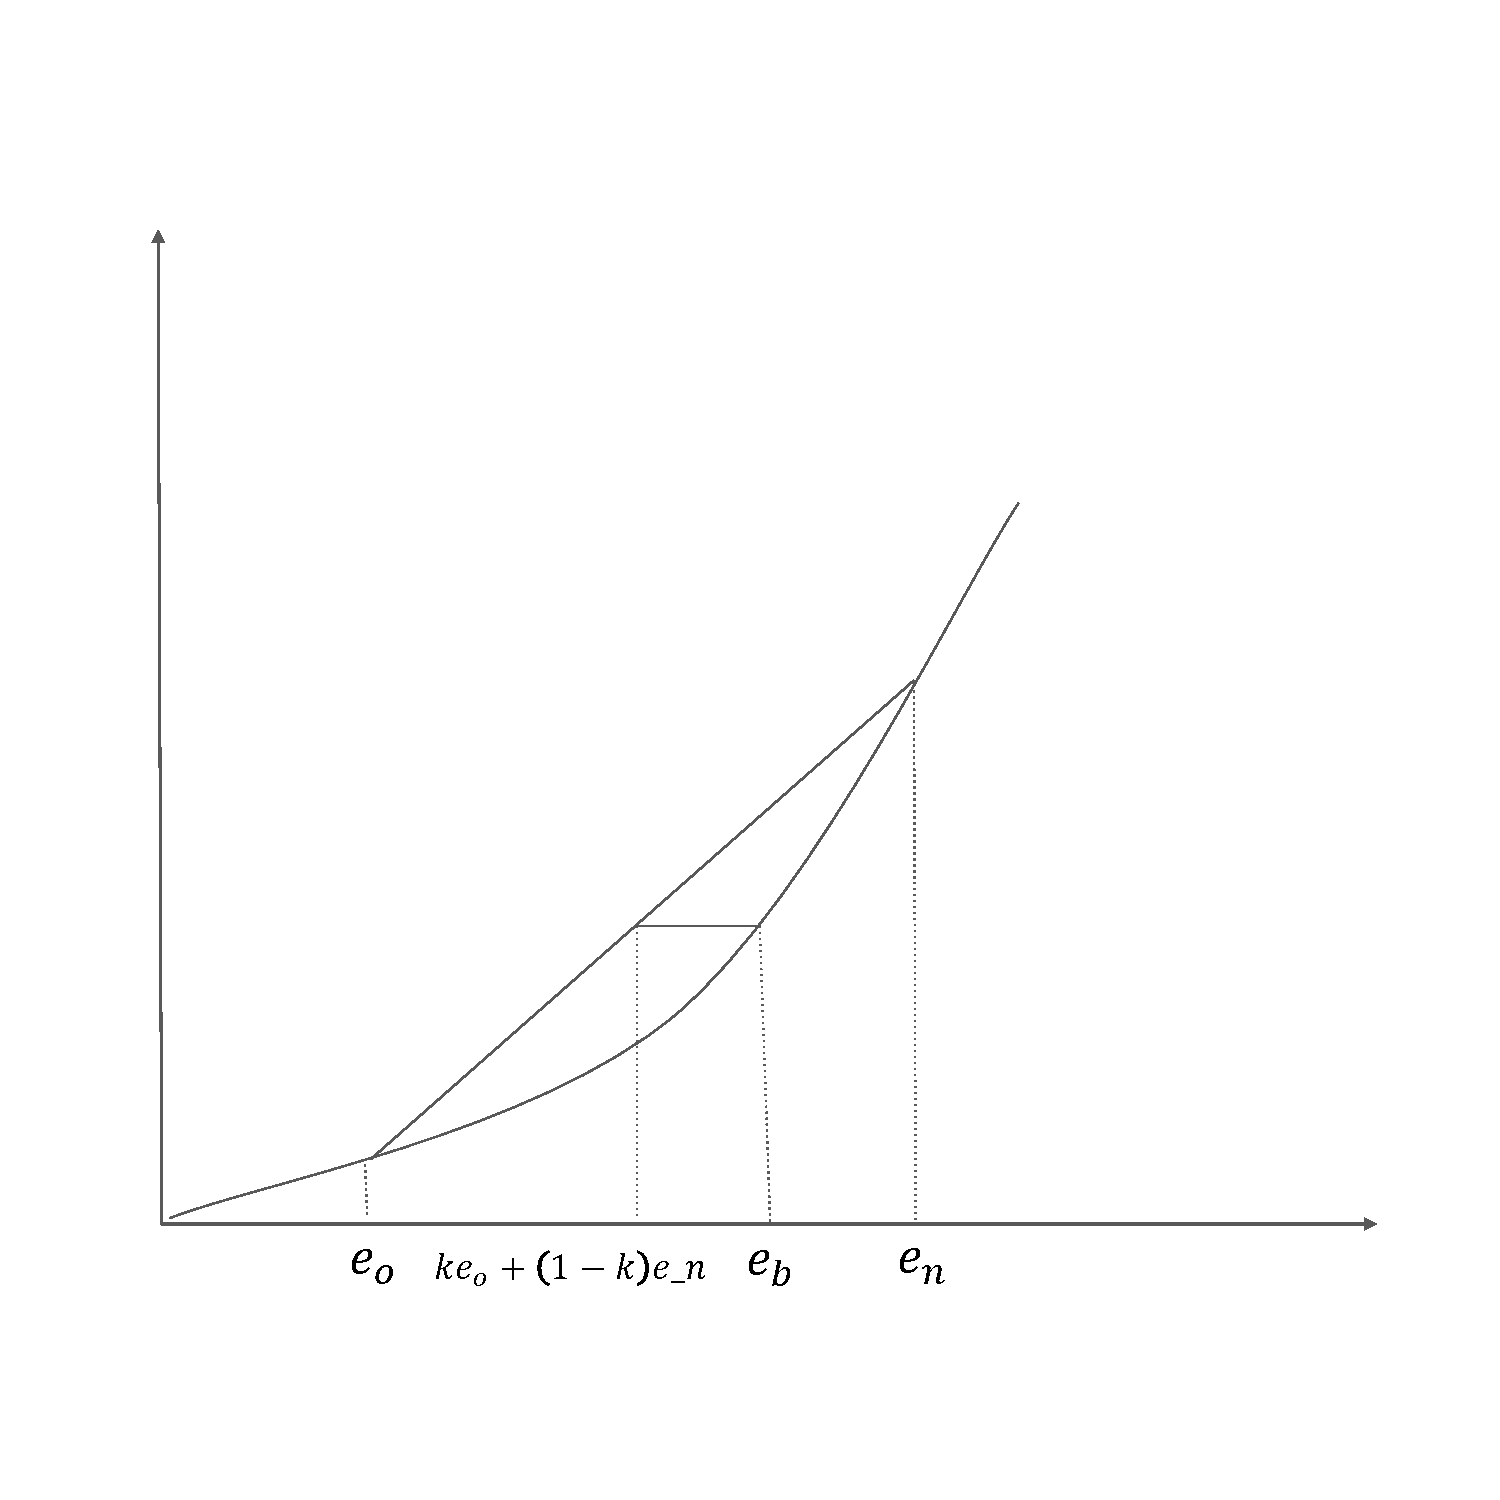
\includegraphics[width=\textwidth]{../Figures/fig1.pdf}
        \caption{$c(e) = \frac{1}{2}e^2$}
    \end{subfigure}
    % right graphic
    \begin{subfigure}[t]{0.45\textwidth}
        \centering
        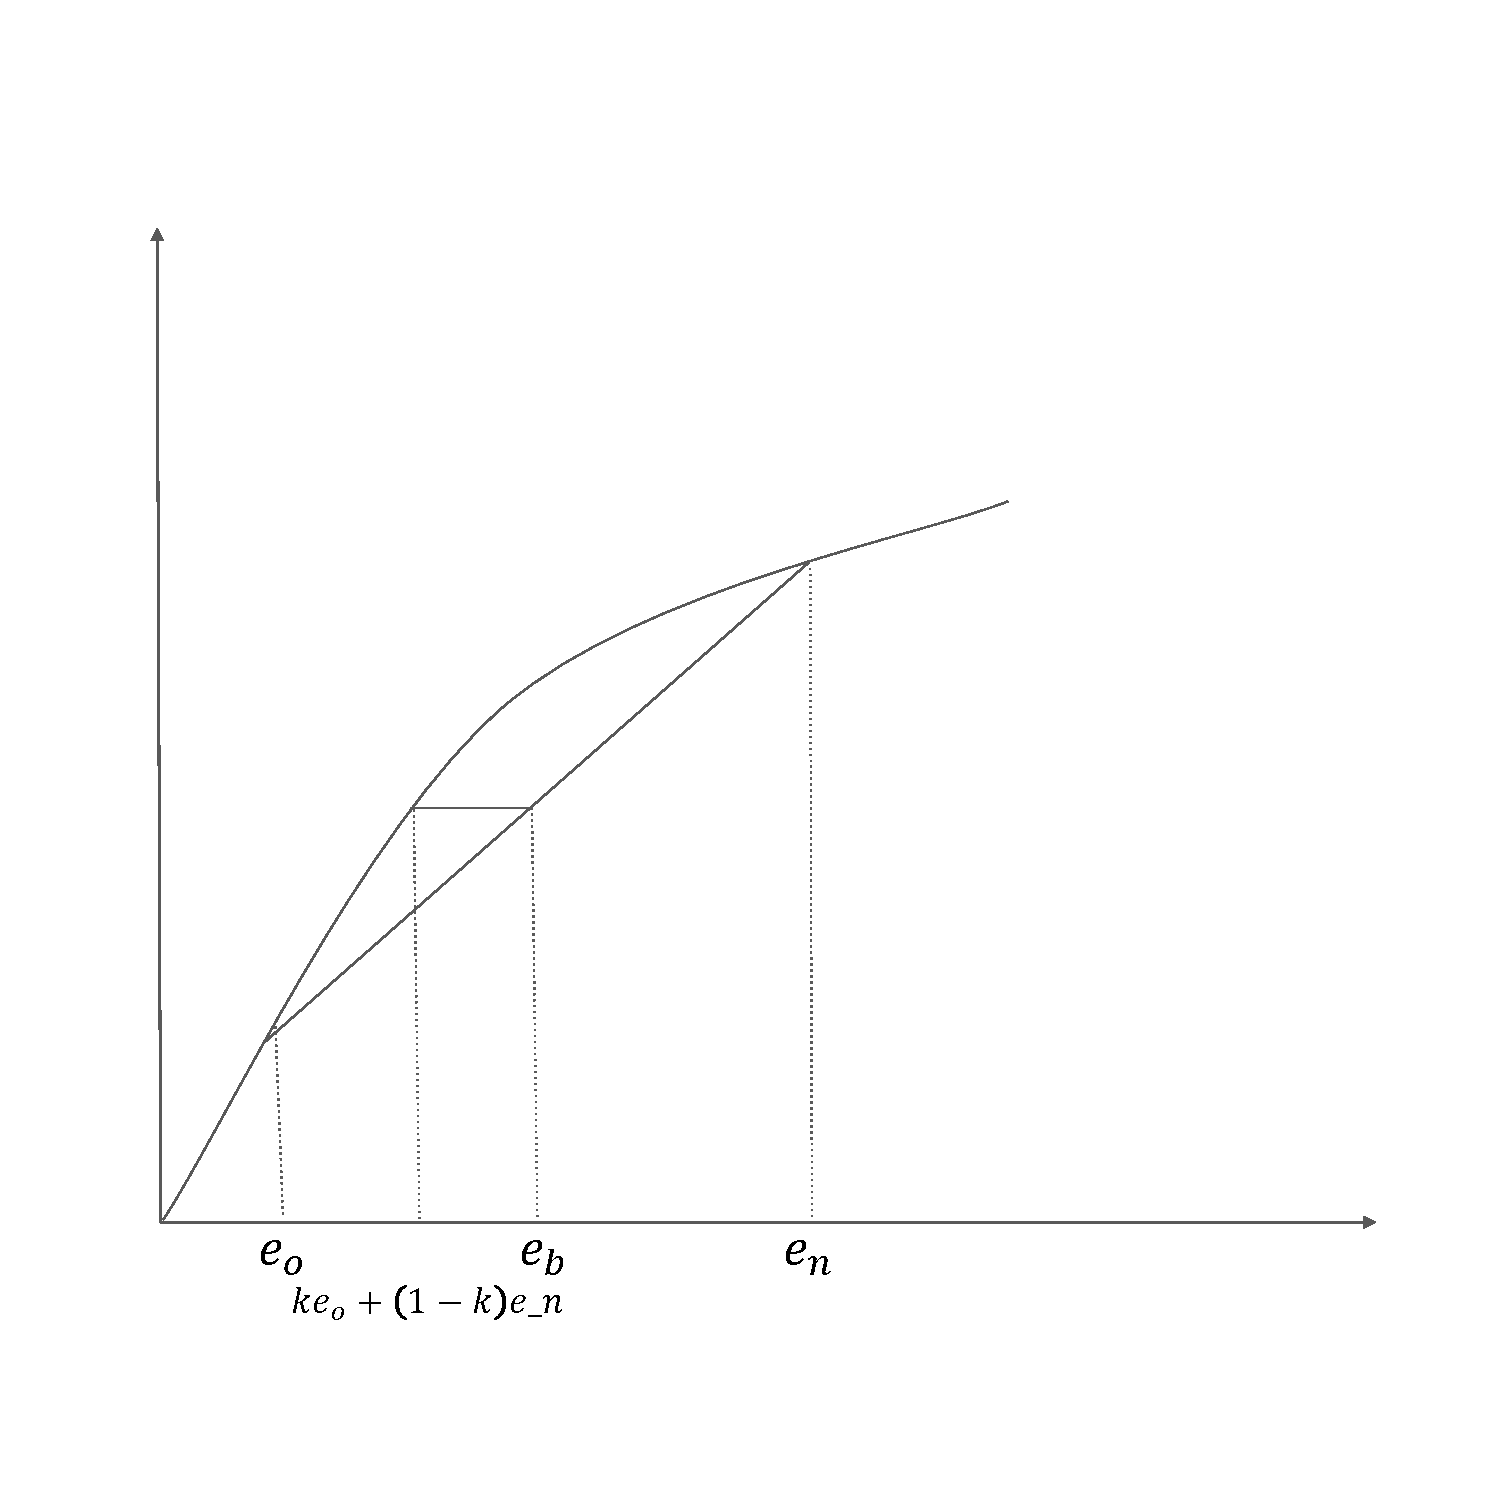
\includegraphics[width=\textwidth]{../Figures/fig2.pdf}
        \caption{$c(e) = \log(e+1)$}
    \end{subfigure}
    \caption{It is the difference between the curvature of the $c(e)$ and $p(e)$ that matters. This figure is only illustrative.}
    \label{fig:cost_function}

\end{figure}

\begin{proposition}
    If $c''(e) \geq p''(e)$ for all $e$, the editor always prefers the double-blind mechanism, subject to a status quo level of anonymity $\lambda_{sq}$. However, when this condition does not hold, and the differences in author productivity and reviewer biases are not too large, the editor may prefer the single-blind mechanism.
\end{proposition}

While I initially expected that the status quo anonymity level
$\lambda_{sq}$\footnote{That is, how difficult it is for the paper to remain
    truly anonymous.} would play a role in the editor's decision $\lambda \in
    \set{\lambda_{sq}, 1}$, it turns out that it does not matter at all under the
current model setup. This question is explored in the next section.

\section{Discussion}
In this section, I discuss several aspects of the model that I have considered
but intentionally ignored in the previous section.

\paragraph{Non-Anonymity Level $\lambda_{sq}$}
Several studies provide evidence that in certain research fields, implementing a double-blind review system offers little to no benefit. Since reviewers are typically assigned papers within their own fields, there is a high likelihood that they have already encountered the work as a preprint on an archive, as a working paper, or through attending the author's presentation. This is particularly true for niche research areas. These findings suggest that, intuitively, a higher level of $\lambda_{sq}$ (the status quo non-anonymity level) should favor the single-blind mechanism.

As discussed in Section~\ref{sec:analysis}, the editor will always choose the
double-blind mechanism if full anonymity yields a higher payoff than full
disclosure. However, in practice, full anonymity is rarely achieved, even under
a double-blind system, because there is an inherent level of non-anonymity
$\lambda_{sq}$ for each research field. All else being equal, a research field
where it is easier to maintain true anonymity (i.e., a low $\lambda_{sq}$) is
more likely to adopt a double-blind system, whereas a field where everyone
knows everyone (i.e., a high $\lambda_{sq}$) is more likely to adopt a
single-blind system.

To incorporate this intuition into the model, I propose introducing a fixed
anonymization cost $c$ for the editor when implementing a double-blind
mechanism. This cost represents the additional effort required to anonymize
papers\footnote{This includes more than just removing author names; it also
    involves verifying that no identifying information is inadvertently included in
    the submission.}. The fixed cost is assumed to be the same across all fields.

Therefore, even if:
\begin{equation*}
    \begin{split}
        \alpha p_1(e_b) + \tau(1-\alpha)p_0(e_b)> &
        k\beta_o p_1(e_o) + (1-k)\beta_n p_1(e_n)   \\ & + \tau(k(1-\beta_o)p_0(e_o) + (1-k)(1-\beta_n)p_0(e_n))\\
                                                  &
        \underbrace{-k\tau b_o(1-\beta_o) - (1-k)\tau b_n\beta_n }_{\text{bias}}
    \end{split}
\end{equation*}
the fixed anonymization cost may be large enough to make the double-blind mechanism unappealing if the weight $(1 - \lambda_{sq})$ on the larger term $\alpha p_1(e_b) + \tau (1 - \alpha) p_0(e_b)$ is small.

By incorporating a fixed anonymization cost into the model, the editor's choice
of mechanism becomes dependent on the status quo non-anonymity level
$\lambda_{sq}$, as desired.

\paragraph{Reviewer's Indifference Condition}
I have assumed that the reviewer is indifferent between the two mechanisms
since they do not receive any compensation or reward for their time spent, as
is the case in reality. This indifference condition serves as a constraint in
the combined problem \ref{eq:combined}. However, I argue that this condition
alone is not sufficient to pin down the effort levels $(e_b, e_o, e_n)$ given
all the parameters specified earlier. This is because, for either $\lambda \in
    \set{\lambda_{sq}, 1}$, the editor's payoff is maximized when the reviewer's
effort is as high as possible. Yet there is no constraint on the upper bound of
$c(e)$. To address this, an additional constraint should be imposed, such as:
\[
    k c(e_o) + (1 - k) c(e_n) < \bar{c},
\]
so that all decision variable $\lambda, e_b, e_o, e_n$ can be pinned down.

Another potential extension is to introduce the reviewer's incentives in their
effort decision. Currently, both mechanisms \textit{blind} the reviewer's
identity, meaning they receive only a generic acknowledgment such as, "We thank
the anonymized reviewers for their helpful feedback." It would be interesting
to explore ways to reward reviewers in non-pecuniary ways such as implementing
a reputation system \citep{soergel2013open}. Alternatively, we could imagine a
world where the reviewer's feedback is openly accessible, or even where the
reviewer's identity is disclosed. If reviewers are incentivized in some way,
the original question takes on the flavor of a classical principal-agent
problem. In that case, the editor (principal) would need to juggle multiple
factors in her choice of mechanism.

\paragraph{Editor's Objective Function}
I have briefly alluded to the four types of outcomes that concern the editor,
as shown in Table~\ref{tab:editor_objective}. Intuitively, the editor seeks to
maximize the diagonal terms (correct acceptance and correct rejection) while
minimizing the off-diagonal terms (false acceptance and false rejection). I
argue that it is sufficient to focus on two out of the four outcomes, provided
that a countervailing pair is selected, such as $h_i \delta_i$ and $-\delta_i$.
By labeling the elements in the table horizontally, I can select pairs such as
$(1, 2)$, $(1, 4)$, $(2, 4)$, $(2, 3)$, or $(4, 3)$. Alternatively, considering
only $(4)$ also works if I attach equal importance to the two objectives
(accept good and reject bad).

\paragraph{Concluding words} In this research proposal, I model the journal editor's choice between
double-blind and single-blind peer review mechanisms, assuming the reviewer
spends a fixed amount of time on reviewing. The peer review process is framed
as a tool to discover paper quality rather than improve it, with the reviewer
exhibiting bias toward two author types. I birefly explore the conditions under
which the editor prefers one mechanism over the other and discuss how a fixed
anonymization cost can make the choice dependent on the field's status quo
non-anonymity level.

\pagebreak
\newpage
\bibliography{../References/ref.bib}

\end{document}